\documentclass[tikz]{standalone}

\usepackage{xcolor}

\definecolor{stgoblue}{RGB}{74,144,226}
\definecolor{stgogreen}{RGB}{80,227,194}
\definecolor{stgored}{RGB}{255,69,0}

\usetikzlibrary{calc}

\begin{document}

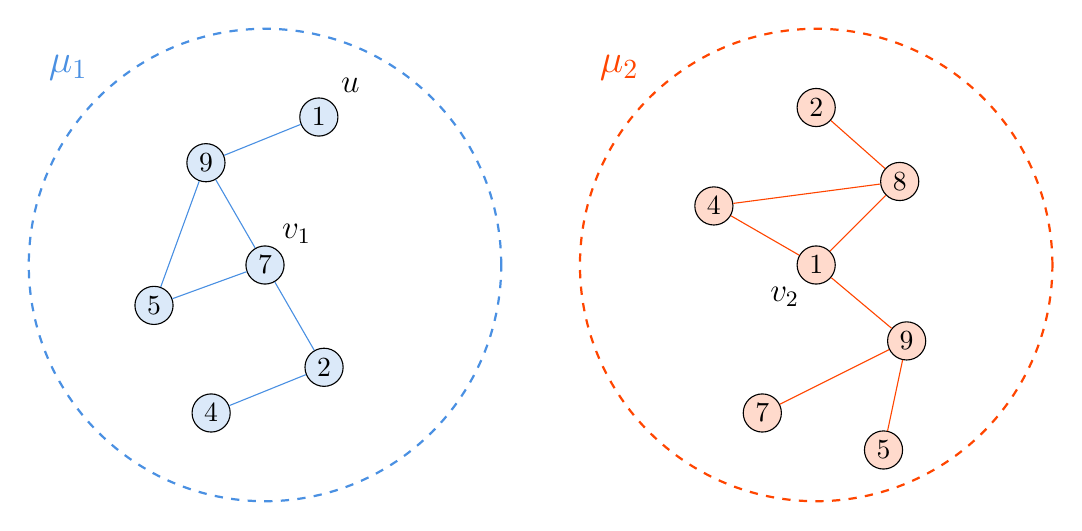
\begin{tikzpicture}
    % Node styles
    \tikzstyle{nodeStyle}=[circle, draw, fill=white, inner sep=2pt]

    % Colors
    \colorlet{uColor}{stgoblue}
    \colorlet{vColor}{stgored}

    % Draw centers
    \node[nodeStyle, fill=uColor!20] (u) at (0,0) {$7$};
    \node[nodeStyle, fill=vColor!20] (v) at (7,0) {$1$};

    % Draw u neighborhood
    \draw[thick, dashed, uColor] (u) circle (3cm);

    % Draw v neighborhood
    \draw[thick, dashed, vColor] (v) circle (3cm);

    % Draw nodes and edges in u's neighborhood
    \node[uColor] (mu1) at (-2.5,2.5) {\Large $\mu_1$};
    \node (v1label) at (0.4,0.4) {\large $v_1$};
    \node[nodeStyle, fill=uColor!20] (u1) at (120:1.5) {$9$};
    \node[nodeStyle, fill=uColor!20] (u2) at (300:1.5) {$2$};
    \node[nodeStyle, fill=uColor!20] (u3) at (200:1.5) {$5$};
    \node[nodeStyle, fill=uColor!20] (u4) at (250:2) {$4$};
    \node[nodeStyle, fill=uColor!20] (u5) at (70:2) {$1$};
    \node (ulabel) at ($(70:2)+(0.4,0.4)$) {\large $u$};

    \foreach \i in {1,...,3} {
        \draw[uColor] (u) -- (u\i);
    }
    \draw[uColor] (u2) -- (u4);
    \draw[uColor] (u1) -- (u3);
    \draw[uColor] (u1) -- (u5);

    \begin{scope}[shift={(7,0)}]
      % Draw nodes and edges in v's neighborhood
      \node[vColor] (mu2) at (-2.5,2.5) {\Large $\mu_2$};
      \node (vlabel) at (-0.4,-0.4) {\large $v_2$};
      \node[nodeStyle, fill=vColor!20] (v1) at (45:1.5) {$8$};
      \node[nodeStyle, fill=vColor!20] (v2) at (150:1.5) {$4$};
      \node[nodeStyle, fill=vColor!20] (v3) at (320:1.5) {$9$};
      \node[nodeStyle, fill=vColor!20] (v4) at (90:2) {$2$};
      \node[nodeStyle, fill=vColor!20] (v5) at (250:2) {$7$};
      \node[nodeStyle, fill=vColor!20] (v6) at (290:2.5) {$5$};

      \foreach \i in {1,...,3} {
          \draw[vColor] (v) -- (v\i);
      }
      \draw[vColor] (v1) -- (v2);
      \draw[vColor] (v1) -- (v4);
      \draw[vColor] (v3) -- (v5);
      \draw[vColor] (v3) -- (v6);
    \end{scope}
\end{tikzpicture}

\end{document}
